% ------------------------------------------------------------------------
\chapter{Git Helper}

Git creates and maintains a database that store versions of a repository, i.e. versions of a folder.
To create this database for a specific folder the Git application must be installed on the computer. Open the Git console program and go to the specific folder and execute the following command:
\\[0mm]
\par\textbf{git init}
\\[5mm]
The Git database is created and stored in the folder \emph{.git} in the root of your repository. The Git commands allow you to manipulate this database.

\section{Data Model}

To understand Git is fundamental to understand the Git data model.
\begin{figure}[h!]
  \centering
  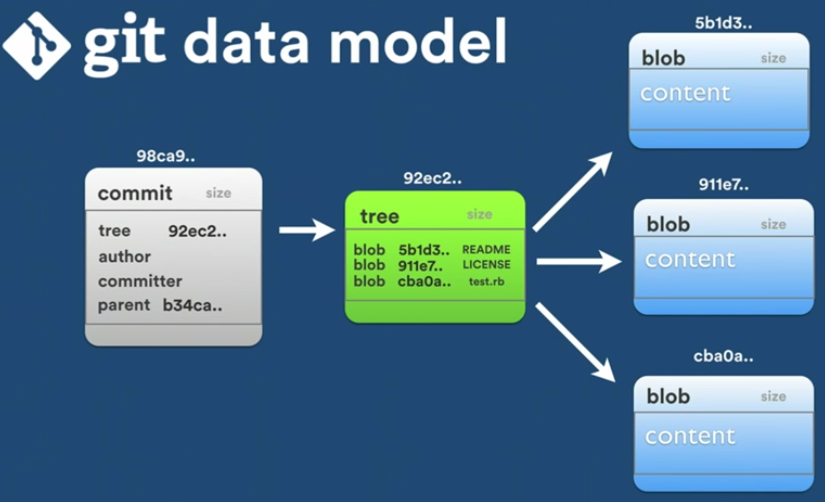
\includegraphics[width=12cm]{../chapter/git/figures/git_data_model.png}
  \caption{Git data model.}\label{git_data_model}
\end{figure}

Git manipulates the following objects:

\begin{itemize}
    \item[\textbullet] {commits - text files that store a description of the repository;}
    \item[\textbullet] {trees - text files that store a description of a folder;}
    \item[\textbullet] {blobs - the files that exist in your repository.}
\end{itemize}
%
\noindent The objects are stored in the folder \emph{.git/objects}. Each store object is identified by its SHA1 hash value, i.e. 20 bytes which identifies unequivocally the object. Note that 20 bytes can be represented by a 40 characters hexadecimal string. The identifier of each object is the 40 characters hexadecimal string. Each particular object is stored in a sub-folder inside the \emph{.git/objects}. The name of the sub-folder is the two most significative characters of the SHA1 hash value. The name of the file that is inside the sub-folder is the remanning thirty eight characters of the SHA1 hash value. The Git stores all committed versions of a file. The Git maintains a contend-addressable file systems, i.e. a file system in which the files can be accessed based on its contend.

A commit object is identified by a SHA1 hash value, and has the following information: a pointer for a tree (the root of your repository), a pointer for the previous commit, the author of the commit, the committer and a commit message.
The author is the person who did the work. The committer is the person who validate the work and who apply the work by doing the commit. By doing this difference git allow both to get the credit, the author and the committer. Example of a commit file contend:\\
\\
tree 2c04e4bad1e2bcc0223239e65c0e6e822bba4f16\\
parent bd3c8f6fed39a601c29c5d101789aaa1dab0f3cd\\
author NetXPTO <netxpto@gmail.com> 1514997058 +0000\\
committer NetXPTO <netxpto@gmail.com> 1514997058 +0000\\
\\
Here goes the commit message.\\

A tree object is identified by a SHA1 hash value, and has a list of blobs and trees that are inside that tree.
Example of a tree file contend:\\
\\
\begin{tabular}{l l l l}
100644 & blob & bdb0cabc87cf50106df6e15097dff816c8c3eb34 &   .gitattributes\\
100644 & blob & 50492188dc6e12112a42de3e691246dafdad645b &   .gitignore\\
100644 & blob & 8f564c4b3e95add1a43e839de8adbfd1ceccf811 &   bfg-1.12.16.jar\\
040000 & tree & de44b36d96548240d98cb946298f94901b5f5a05 &   doc\\
040000 & tree & 8b7147dbfdc026c78fee129d9075b0f6b17893be &   garbage\\
040000 & tree & bdfcd8ef2786ee5f0f188fc04d9b2c24d00d2e92 &   include\\
040000 & tree & 040373bd71b8fe2fe08c3a154cada841b3e411fb &   lib\\
040000 & tree & 7a5fce17545e55d2faa3fc3ab36e75ed47d7bc02 &   msbuild\\
040000 & tree & b86efba0767e0fac1a23373aaf95884a47c495c5 &   mtools\\
040000 & tree & 1f981ea3a52bccf1cb00d7cb6dfdc687f33242ea &   references\\
040000 & tree & 86d462afd7485038cc916b62d7cbfc2a41e8cf47 &   sdf\\
040000 & tree & 13bfce10b78764b24c1e3dfbd0b10bc6c35f2f7b &   things\_to\_do\\
040000 & tree & 232612b8a5338ea71ab6a583d477d41f17ebae32 &  visualizerXPTO\\
040000 & tree & 1e5ee96669358032a4a960513d5f5635c7a23a90 &   work\_in\_progress\\
\end{tabular}
\\
A blob is identified by a SHA1 hash value, and has the file contend compressed. A git header and tailor is added to each file and the file is compressed using the zlib library. The git header is just the file type, file size and the \textbackslash NUL caracter, for instance "blob 13\textbackslash NUL", the tailor is just the \textbackslash n caracter. The blob is stored as a binary file.

\section{Refs}

SHA1 hash values are hard to memorize by humans. To make life easier to humans we use refs. A ref associate a name, easier to memorize by humans, with a SHA1 hash value. Therefore refs are pointers to objects. Refs are implementes by text files, the name of the file is the name of the ref and inside the file is a string with the SHA1 hash value.

There are different type of refs. Some are static, for instance the tags, others are actualized automatically, for instance the branches.

\section{Tags}

A tag is just a ref for a specific commit. A tag do not change over time.

\section{Branch}

A branch is a ref that points for a commit that is originated by a divergence from a common point.
A branch is automatically actualized so that it always points for the most recent commit of that branch.

\section{Heads}

Heads is a pointer for the commit where you are.

\section{Database Folders and Files}

\subsection{Objects Folder}

Git stores the database and the associated information in a set of folders and files inside the the folder \emph{.git} in the root of your repository.

The folder \emph{.git/objects} stores information about all objects (commits, trees and blobs).
The objects are stored in files inside folders.
The name of the folders are the 2 first characters of the SHA1 40 characters hexadecimal string.
The name of the files are the other 38 hexadecimal characters of the SHA1.
The information is compressed to save same space but it can be access using some applications.

\subsection{Refs Folder}

The \emph{.git/refs} folder has inside the following folders \emph{heads},\emph{remotes}, and \emph{tags}.
The \emph{heads} has inside a ref for all local branches of your repository.
The \emph{remotes} folder has inside a set of folders with the name of all remote repositories, inside each folder is a ref for all branches in that remote repository.
The \emph{tag} folder has a ref for each tag.

\section{Git Spaces}

Git uses several spaces.

\begin{itemize}
    \item[\textbullet] {workspace - is your directories where you are working;}
    \item[\textbullet] {index - when you record changes before commit them;}
    \item[\textbullet] {blobs - the files that exist in your repository.}
\end{itemize}



\begin{figure}[h!]
  \centering
  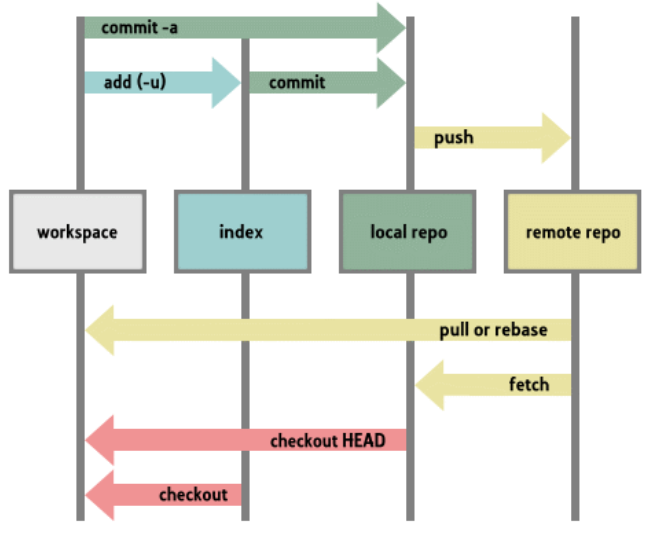
\includegraphics[width=12cm]{../chapter/git/figures/git_spaces.png}
  \caption{Git spaces.}\label{git_spaces}
\end{figure}


\section{Workspace}

\section{Index}

\section{Merge}

Merge is a fundamental concept to git. It is the way you consolidate your work.

\subsection{Fast-Forward Merge}

\subsection{Resolve}

\subsection{Recursive}

\subsection{Octopus}

\subsection{Ours}

\subsection{Subtree}

\subsection{Custom}

\section{Commands}


\subsection{Porcelain Commands}

\textbf{git add}

\noindent \emph{git add}, store a file that was changed to the index.


\noindent \textbf{git bisect}

\noindent \textbf{git branch}

\noindent \emph{git branch --set-upstream-to=<remote>/<branch> <local branch>}, links a local branch with a branch in a remote repository.


\textbf{git cat-file}

git cat-file -t <hash>

shows the type of the objects

git cat-file -p <hash>

shows the contend of the object

\textbf{git clone}

\textbf{git diff}

\emph{git diff} shows the changes in the working space.

\emph{git diff --name-only} shows the changes in the working space, only file names.

\emph{git diff --cached} shows the changes in the index space.

\emph{git diff --cached --name-only} shows the changes in the index space, only file names.

\textbf{git fecth -all}


\noindent \textbf{git init}

\emph{git init}, used to initialize a git repository. It creates the \emph{.git} folder and all its subfolders and files.
The subfolders are \emph{objects}, \emph{refs}, ... There are also the following files \emph{HEAD}.

\textbf{git log}

shows a list of commits from reverse time order (goes back on time), i.e. shows the history of your repository. The history of a repository can be represented by a directed acyclic graph (dag for short), pointing in the forward direction in time.

options

--graph

 shows a graphical representation of the repository commits history.

\noindent \textbf{git rebase}

\emph{git rebase <branch2 or commit2>}, finds a common point between the current branch and branch2 or commit2, reapply all commits of your current branch from that divergent points on top of branch2 or commit2, one by one.

\noindent \textbf{git reset}

\emph{git reset --soft HEAD~1}, moves one commit back but keeps all modified files.

\emph{git reset --hard HEAD~1}, moves one commit back and cleans all the modified files.

\textbf{git reflog}

Keep a log file with all commands from the last 90 days.

\textbf{git show}

Shows what is new in the last commit.

\noindent \textbf{git stash}

Stash is a global branch where you can store the present state.

\emph{git stash}, save the present state of your repository.

\emph{git stash --list}, shows what is in the stash.

\textbf{git status}

\subsection{Pluming Commands}

\noindent \textbf{git count-object}

\emph{git count-object -H}, counts all object and shows the result in a readable form (-H, human).

\textbf{git gc}

Garbage collector.
Eliminates all objects that are not referenced, i.e. has no reference associated with.

git gc --prune=all


\noindent \textbf{git hash-object}

\emph{git hash-object -w <file>}, calculates the SHA1 hash value of a file and write it in the \emph{.git/objects} folder.

\noindent \textbf{git cat-files}

\emph{git cat-files -p <sha1>}, shows the contend of a file in a readable format (flag -p, pretty format).

\emph{git cat-files -t <sha1>}, shows the type of a file.

\noindent \textbf{git update-index}

\emph{git update-index --add <file name>}, creates the hash and adds the <file\_name> to the index.

\noindent \textbf{git ls-files}

\emph{git ls-files --stage}, shows all files that you are tracking.

\noindent \textbf{git write-tree}

\noindent \textbf{git commit-tree}

\noindent \textbf{git update-ref}

\emph{git update-ref refs/heads/<branch name> <commit sha1 value>}, creates a branch that points to the <commit sha1 value>.

\noindent \textbf{git verify-pack}

\section{The Configuration Files}

There is a config file for each repository that is stored in the \emph{.git/} folder with the name \emph{config}.\\
\\
There is a config file for each user that is stored in the \emph{c:/users/<user name>/} folder with the name \emph{.gitconfig}.\\
\\
To open the \emph{c:/users/<user name>/.gitconfig} file type:\\
\\
\textbf{git config --global -e}

\section{Pack Files}

Pack files are binary files that git uses to save data and compress your repository. Pack files are generated periodically by git or with the use of gc command.

\section{Applications}

\subsection{Meld}

%# --------------------------------------D I F F -----------------------------
%
%[diff]
%    guitool = meld
%
%[difftool "meld"]
%    cmd = \"C:/Program Files (x86)/Meld/Meld.exe\" \"$LOCAL\" \"$REMOTE\" --label \"DIFF (ORIGINAL MY)\"
%	
%# --------------------------------------M E R G E -----------------------------
%
%[merge]
%    tool = meld
%
%[mergetool "meld"]
%    cmd = \"C:/Program Files (x86)/Meld/Meld.exe\" --auto-merge \"$LOCAL\" \"$BASE\" \"$REMOTE\" --output \"$MERGED\" --label \"MERGE (REMOTE BASE MY)\"
%    trustExitCode = false
%
%[mergetool]
%    # don't ask if we want to skip merge
%    prompt = false
%
%    # don't create backup *.orig files
%    keepBackup = false

\subsection{GitKraken}

\section{Error Messages}

\subsection{Large files detected}

Clean the repository with the \href{https://rtyley.github.io/bfg-repo-cleaner}{BFG Repo-Cleaner}.\\
\\
Run the Java program:\\

java -jar bfg-1.12.16.jar \texttt{-{}-}strip-blobs-bigger-than 100M\\
\\
This program is going to remote from your repository all files larger than 100MBytes. After do:\\

git push \texttt{-{}-}force.
